\documentclass[a4paper,10pt,fleqn]{article}

\usepackage{layout}

\newboolean{STANDALONE}
\setboolean{STANDALONE}{false}

\newboolean{EMBED}
\setboolean{EMBED}{false}


\setboolean{EMBED}{true}

\title{Dokumentation BLDC}
\newcommand{\BrushlessPath}{src}
\newcommand{\DasAndereTeam}{T27 }
\newcommand{\BLDCTeams}{T27 und T32}
\newcommand{\BLDCcollab}{Dieses Kapitel ist eine Zusammenarbeit der Gruppen \BLDCTeams. }

\begin{document}

\maketitle
\clearpage
\tableofcontents
\clearpage

\ifSTANDALONE
\section{Hardware}
\fi
\ifEMBED
\subsection{Hardware}
\fi
Die Elektrotechnik-Studierenden aus mehreren Gruppen haben sich
zusammengeschlossen um gemeinsame Probleme anzugehen. Dabei handelt es sich
um die benötigte Hard- und Software, um Motoren anzusteuern
und gegebenenfalls zu regeln. In diesem Zusammenschluss wurden drei Gruppen
gebildet, um Lösungen für DC-, Stepper- und Brushless-Motoren auszuarbeiten.
Die Idee besteht darin, dass nicht jede Gruppe für dasselbe Problem wo
möglich denselben Lösungsansatz verfolgt, sondern die Ressourcen kombiniert,
Synergien nutzt um eine bessere Lösung zu erarbeiten. Auf diese Weise kann
das Team übergreifende Arbeiten im Rahmen der PREN erlernt und
geübt werden. Somit wird Idee der Interdisziplinarität im erweiterten Sinn
Rechnung getragen. Die Gruppen und deren Mitglieder sind in der Tabelle 
\ref{tab:pren-et-overview} aufgeführt.
\begin{table}[h!]
	\centering
	\begin{tabular}{l l}
		Projekt		& Team \\
		\hline
		DC Motoren	& 39 \\
		Schrittmotor	& 27, 38 \\
		BLDC Motor	& 27, 32 \\
	\end{tabular}
	\caption{Übersicht der PREN-ET Projektgruppen}
	\label{tab:pren-et-overview}
\end{table}

\newpage
\ifSTANDALONE
\section{Stepper Motoransteuerung}
\fi
\ifEMBED
\subsection{Stepper Motoransteuerung}
\fi

\ifEMBED
    % Dieses Kapitel ist eine Zusammenarbeit der Gruppen \BLDCTeams. 
    \BLDCcollab
\fi
    \ifSTANDALONE
    \subsection{Grundsätzliches zur Ansteuerung}\label{subsec:Ansteuerung}
    \fi
    \ifEMBED
    \subsubsection{Grundsätzliches zur Ansteuerung}\label{subsec:Ansteuerung}
    \fi
    	Grundsätzlich besteht die Ansteuerung aus drei Teilen, wie in \autoref*{fig:ansteuerung} gezeigt. 
    	\begin{figure}[H]
    		\centering
    		
\begin{tikzpicture}
    		\draw[line width=1.5pt](0, 0) rectangle node{Mikrokontroller} (3, 1)  ;
    		\draw[line width=1.5pt, ->]	(3, 0.5) -- (4, 0.5);
    		\draw[line width=1.5pt](4, 0) rectangle node{Steuerung}(7, 1);
    		\draw[line width=1.5pt, ->]	(7, 0.5) -- (8, 0.5);
    		\draw[line width=1.5pt](8, 0) rectangle node{Treibertufen}(11, 1);
    		\end{tikzpicture}
    		\caption{Komponenten der Ansteuerung eines Schrittmotores}
    		\label{fig:ansteuerung}
    	\end{figure}
        Um die Ansteuerung zu realisieren, gibt es eine Vielzahl von integrierten Schaltkreisen. Diese unterscheiden sich wie folgt: 
        \begin{itemize}
        	\item \textbf{Interfaces:} Einzelanschlüsse, einfache Busschnittstellen oder Mikrokontrollerschnittstellen wie SPI, II2
        	\item \textbf{Steuerfunktionen:} Einzelne Schritte oder Bewegungsabläufe (Motion Control Functiona)
        	\item \textbf{Schaltungsintegration:} Steuerung und Treiberstufe als getrennte Schaltkreise, oder in einem Schaltkreis zusammengefasst. 
        \end{itemize}
        Der gewählte integrierte Schaltkreis ist der L6480 von STMicroelectronics. Dieser wird über die SPI Schnittstelle gesteuert und besitzt eine Motion Contol Engine. Die Treiberstufe wird extern realisiert. (Vgl. Kapitel \ref{sec:L6480} 
        
    \ifSTANDALONE
    \subsection{Treiberstufe}
    \fi
    \ifEMBED
    \subsubsection{Treiberstufe}
    \fi 
    	Wird ein Schrittmotor unipolar betrieben, so können die vier Wicklungen direkt mit Leistungsstufen angesteuert werden. Für den bipolaren Betrieb benötigt man für beide Wicklungen je eine H- Brücke. Die einfachste Methode ist es, den Strom nur durch den Wicklungswiderstand zu begrenzen. Der Nachteil ist, dass die Zeitkonstante durch den Wicklungswiderstand und der Induktivität bestimmt ist, und so bei höheren Schrittfrequenzen der gewünschte Strom und damit das Drehmoment nicht mehr erreicht wird. Deshalb wird ein zusätzlicher Vorwiderstand in Serie geschaltet, und so die Zeitkonstante verkleinert. Typische Verhältnisse sind vierfacher- oder fünffacher Widerstand, was eine vierfache bzw. fünffache Speisespannung voraussetzt. Diese Methode wiederum führt zu einer höheren Verlustleistung in den Widerständen. Im Ruhezustand ist es sinnvoll, den Strom soweit zu senken, dass das Haltemoment nicht unterschritten wird. Eine Spannungsumschaltung hat den weiteren Vorteil, dass so beim Anfahren eine steilere Stromkurve erreicht werden kann. (Vgl. \autoref{fig:spannungsumschaltung})
    	 \begin{figure}
    	 	\centering
    	 	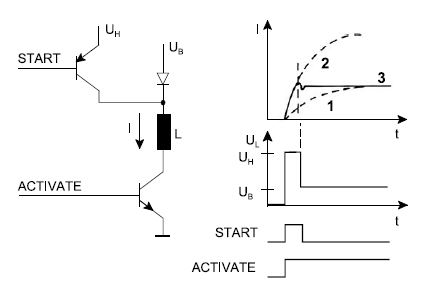
\includegraphics[width=8cm]{\EtPath/Bilder/spannungsumschaltung.JPG}
    	 	\caption{Spannungsumschaltung}
    	 	\label{fig:spannungsumschaltung}
    	 \end{figure}
    	Der Schrittmotor kann alternativ auch stromgesteuert betrieben werden. Dabei folgt der Stromverlauf dem Verlauf einer Referenzspannung (Sollwert). Der Stromverlauf wird auf den Sollwert geregelt. Die Betriebsspannung muss so nicht stabilisiert werden. \label{stromgesteuert} 
	
	
		
\newpage
\ifSTANDALONE
\section{Prinziptest}
\fi
\ifEMBED
\subsubsection{Aufbaubeschreibung}
    \BLDCcollab
\fi
\ifEMBED
    \begin{wrapfigure}{r}{0.55\textwidth}
       	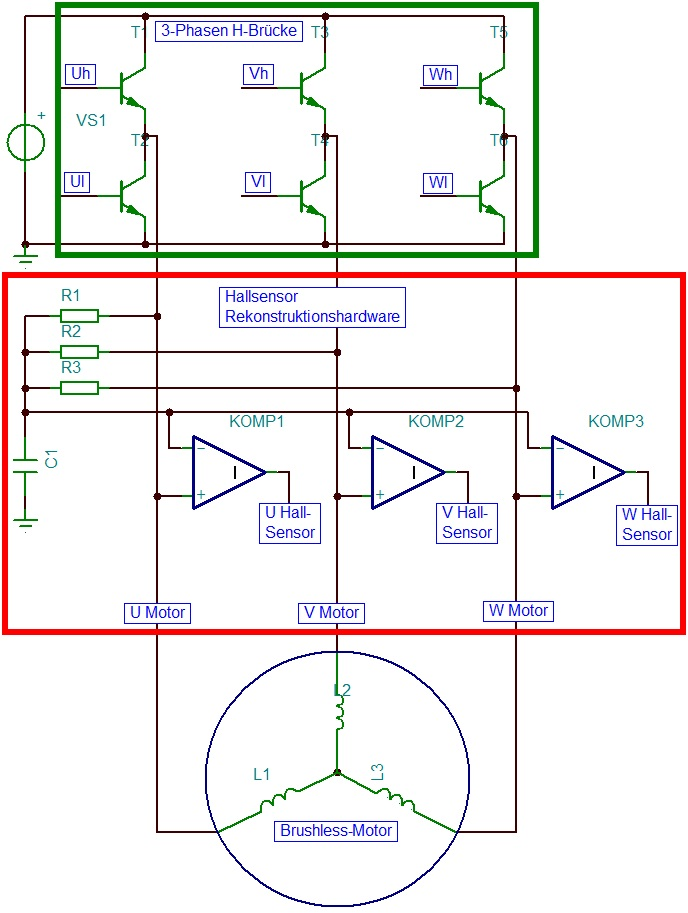
\includegraphics[scale=0.4]{\EtPath/Bilder/MotoransteuerungSchema.jpg}
       	\centering
       	\caption{Schema des Brushless-Versuchsaufbaus}
        \label{abb:MotoransteuerungSchema}
    \end{wrapfigure}
\fi
    Das Schema des Gesamtaufbaus des Tests ist in der Abbildung 
    \ref{abb:MotoransteuerungSchema} ersichtlich. Die 3-Phasen H-Brücke 
    im oberen grünen Rechteck wird direkt vom FPGA angesteuert. Die Hardware 
    dieser Brücke ermöglicht eine voll galvanisch getrennte Ansteuerung 
    mit 3.3V Logikpegeln. Diese Brücke wurde zur Verfügung gestellt und direkt
    implementiert. Die Rekonstruktion der Hallsensoren-Signale findet im rot 
    markierten Teil des Aufbaus statt. Dieser Part wurde auf einer 
    Laborplatte aufgebaut und gelötet. Die so generierten Signale 
    $U_{Hallsensor}$, $V_{Hallsensor}$, $W_{Hallsensor}$ werden einem FPGA 
    geliefert. Anhand dieser Signale steuert das FPGA die 
    H-Brücken-Transistoren mit den Signalen $U_h$, $U_l$, $V_h$, $V_l$, 
    $W_h$, $W_l$. Die im FPGA enthaltene Konfiguration besteht aus simplen 
    AND-Verknüpfungen, die die anliegenden Signale sehr schnell und 
    effizient verarbeiten können. Auf diese Weise ist es möglich, den Motor sehr 
    schnell anzusteuern.
    \ifSTANDALONE
    \begin{figure}[h!]
    	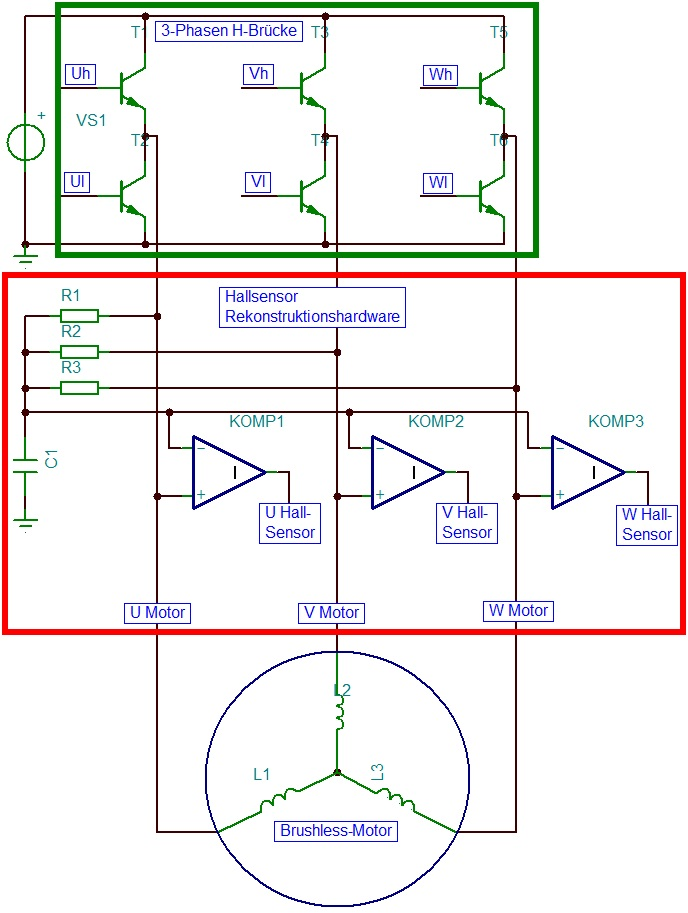
\includegraphics[scale=0.4]{\EtPath/Bilder/MotoransteuerungSchema.jpg}
       	\centering
       	\caption{Schema des Brushless-Versuchsaufbaus}
        \label{abb:MotoransteuerungSchema}
    \end{figure}
    \fi
    In der Abbildung \ref{abb:MessplatzAufbau} ist der gesamte Aufbau 
    abgebildet. Man beachte die markierten Felder. Am linken unteren Rand 
    ist der Motor befestigt. In der Mitte des Bildes ist die Hardware zur Rekonstruktion der Hallsensoren-Signale.
    Die generierten Signale werden dem FPGA in der unteren linken Ecke zugeführt. Diese 
    Signale werden logisch verknüpft und danach die sechs Signale 
    generiert, um die H-Brücke in der rechten oberen Hälfte anzusteuern. 
    Die H-Brücken wiederum treiben den Motor an.
    \begin{figure}[h!]
    %\vspace{-16pt}
       	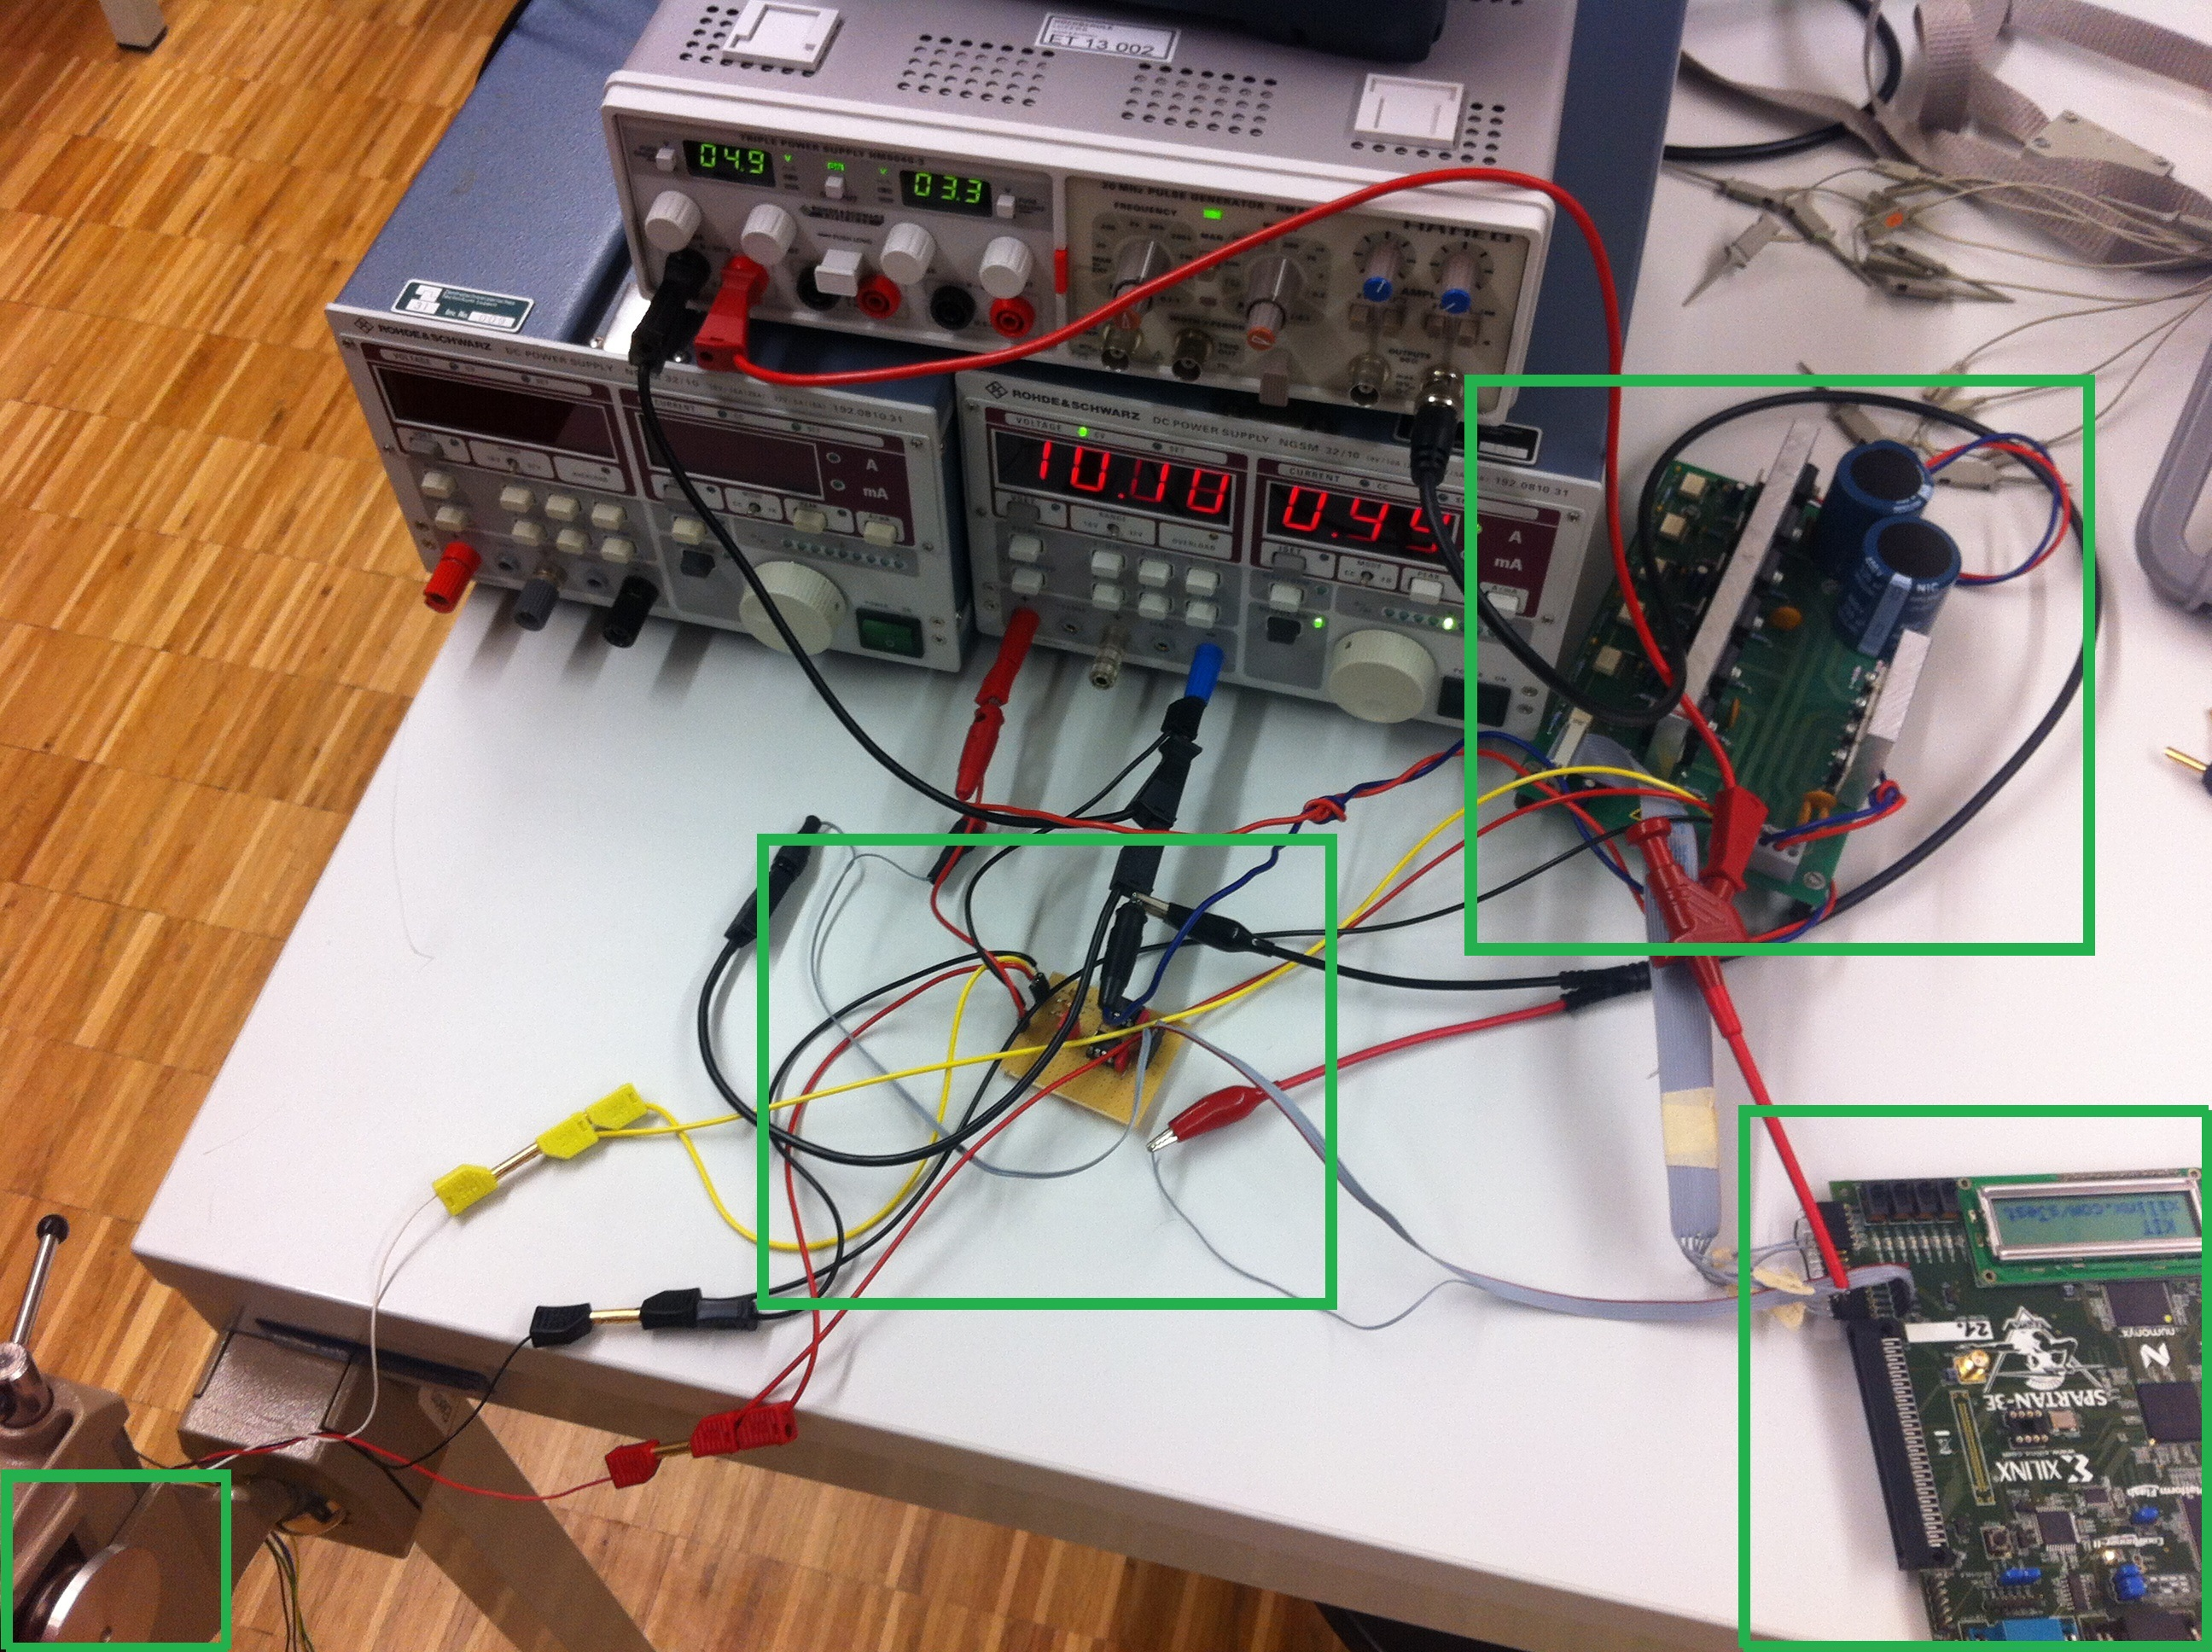
\includegraphics[scale=0.14]{\EtPath/Bilder/MessplatzAufbau.jpg}
       	\centering
       	\caption{Testaufbau} 
        \label{abb:MessplatzAufbau}
    %\vspace{-10pt}
    \end{figure}
    Die im FPGA enthaltene Logik basiert auf der Wahrheitstabelle, die in 
    Abbildung \ref{abb:WahrheitstabelleAnsteuerung} abgebildet ist.

\ifSTANDALONE
\subsection{Messmittel}
\fi
\ifEMBED
\subsubsection{Messmittel}
\fi
    \begin{table}[h!]
        \centering
        \begin{zebratabular}{lll}
            \rowcolor{gray}
            Gerät &
                Typ &
                Nummer \\
            Speisegerät & 
                Rohde \& Schwarz NGSM 32/10 &
                Inv.-Nr. 009 \\
            Oszilloskop &
                Agilent MSO6052A &
                Inv.-Nr. 44; S/N: MY44001903 \\
            Mainframe &
                Hameg HM8001-2 &
                SN: 059520046 \\
            Speisegerät &
                Hameg HM8040-3 &
                SN: 015405014 \\
            Pulsgenerator &
                Hameg HM8035 &
                Inv.-Nr. 44 \\
        \end{zebratabular}
        \caption{Messmittel des Versuchsaufbaus}
    \end{table}

\newpage
\ifSTANDALONE
\section{Fallback}
\fi
\ifEMBED
\subsection{Fallback}
\fi
Ist der Einsatz des vorgesehenen BLDC-Treibers nicht möglich, so muss eine
alternative Ansteuerung erfolgen. Eine solche kann mit einer handelsüblichen
Steuerungen aus dem Modellbau erfolgen. Eine solche BLDC-Steuerung ist per
PWM angesteuert, wobei die im Modellbau üblichen Signale gelten, wie in der
Abbildung \ref{fig:rc-pwm} dargestellt.

\begin{figure}[h!]
	\centering
	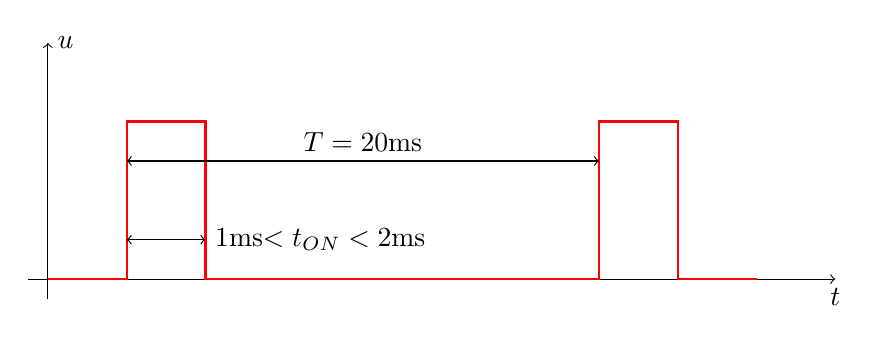
\begin{tikzpicture}
		% Achsen
		\draw[->] (-0.25,0) -- (10,0) node[anchor=north] {$t$};
		\draw[->] (0,-0.25) -- (0,3) node[anchor=west] {$u$};
		% Signal
		\draw[-,red,thick] (0,0) -- (1,0) -- (1,2) -- (2,2) -- 
			(2,0) -- (7,0) -- (7,2) -- (8,2) -- (8,0) -- (9,0);
		% Zeiten
		\draw[<->] (1,1.5) -- (7,1.5) node[midway, above] {$T=20$ms};
		\draw[<->] (1,0.5) -- (2,0.5) node[right] {$1$ms$<t_{ON}<2$ms};
	\end{tikzpicture}
	\caption{Signalverlauf eines typischen Modellbau-PWM Signals}
	\label{fig:rc-pwm}
\end{figure}

Der Einsatz von Modellbausteuerungen für BLDC-Motoren erfordert ein
Feedback der Drehzahl, da diese lediglich eine Steuerung darstellen. Die
Drehzahlregelung muss über eine externe Einheit erfolgen, beispielsweise einen
Mikrocontroller. Solche BLDC-Steuerungen werden im Modellbau typischerweise als
\emph{Regler} vertrieben und sind auch für hohe Leistungen durchaus preiswert.

\ifSTANDALONE
\subsection{Konzeptbeschreibung}
\fi
\ifEMBED
\subsubsection{Konzeptbeschreibung}
\fi
Um eine Regelung der Drehzahl des BLDC-Motors zu ermöglichen, bedarf es eines
Feebacks, welches die Drehzahl wiedergibt. Dies ist mit einem
Hall-Effekt-Schalter zu realisieren. Dieser reagiert auf die Magnetfelder,
welche durch Magnete auf dem Rotationskörper gegeben sind. Aus solch einem
Aufbau resultiert ein Feedback, welches mit Impulsen einen Segmentdurchlauf
des Rotationskörpers wiedergibt, wie in Abbildung \ref{fig:fallback-sketch}
dargestellt.
\begin{figure}[h!]
	\centering
	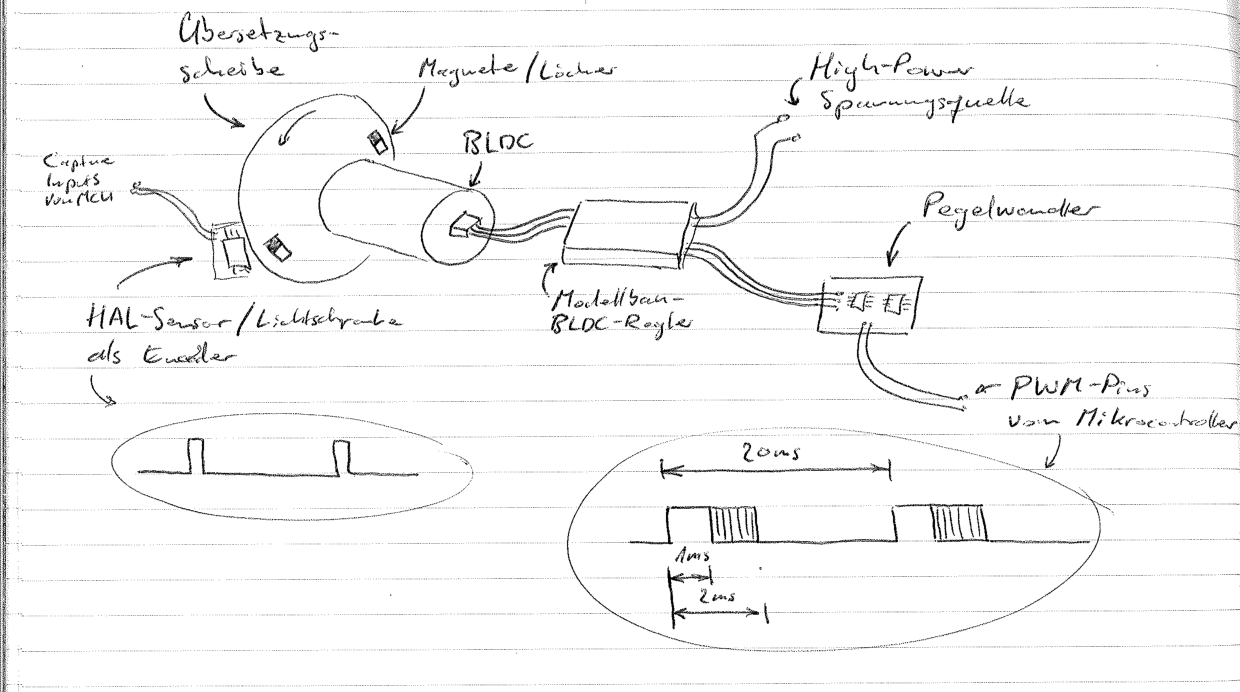
\includegraphics[width=0.8\textwidth]{\EtPath/Bilder/fallback_sketch_1.pdf}
	\caption{Erste Skizze des Fallback-Konzepts}
	\label{fig:fallback-sketch}
\end{figure}
Dieses Feedback wird mittels eines Mikrocontrollers ausgewertet und regelt
damit den Input der Steuerung mit dem PWM-Signal beziehungsweise der Impulsdauer.
Das Einlesen einer Flanke, die Zeitmessung bis zur nächsten Flanke und die
Stellung eines PWM-Signals, sind Tasks welche übliche Mikrocontroller direkt
durch ihre Peripherie-Module ausführen können. Dies ermöglicht eine einfache
Adaption in ein bestehendes Modell, denn es werden lediglich zwei Timer-IO
für diesen Fallback verwendet. Je nach Mikrocontroller ist ein Pegelwandler
für die PWM-Signale notwendig.

\newpage
\ifSTANDALONE
\section{Encoder \& Drehzahlgeber}
\fi
\ifEMBED
\subsubsection{Encoder \& Drehzahlgeber}
\fi

Die vorgesehenen Motorfunktionen verlangen lediglich beim Brushlessmotor
nach einem Feedback über die Rotation des Motors, da der Schrittmotor
definiert und fein granuliert betrieben wird. Der Gleichstrommotor stellt
keinerlei Ansprüche, weder an die Drehzahl, noch an die Position.

Encoder sind relativ teuer und der Einsatz des Brushlessmotors verlangt
lediglich nach einem Feedback zur Rotation beziehungsweise Winkelgeschwindigkeit.
Die absolute oder relative Position ist für die Anwendung nicht von
Bedeutung. Somit lässt sich ein einfaches Feedback vorsehen, für die
Regelung der Drehzahl mit optischen oder magnetischen Elementen.
\ifSTANDALONE
\begin{figure}[h!]
	\centering
	\begin{tikzpicture}
		% Koordinaten
		\draw[->] (-0.5, 0) -- (8, 0) node[anchor=north] {$t$};
		\draw[->] (0, -1.5) -- (0, 3) node[anchor=east] {$u,\varphi$};
		% Rotation
		\draw[blue] (0,0) sin (1,1) cos (2,0) sin (3,-1) cos (4,0)
			sin (5,1) cos (6,0) sin (7,-1)
			node[right] {$\varphi$};
		% Signal
		\draw[-, thick, red]
			(0,0) -- (0.8,0) -- (0.8,2) -- (1.2,2) -- (1.2,0) -- 
			(4.8,0) -- (4.8,2) -- (5.2,2) -- (5.2,0) -- (7.5,0);
		% Messung
		\draw[<->] (0.8,1.5) -- (4.8,1.5) node[midway, above] {$t_{r}$};
	\end{tikzpicture}
	\caption{Vereinfachtes Puls-Feedback eines Hall-Effekt-Schalters}
	\label{fig:hall-effekt-schalter}
\end{figure}
\fi
\ifEMBED
\begin{figure}[h!]
	\centering
	\begin{tikzpicture}
		% Koordinaten
		\draw[->] (-0.5, 0) -- (8, 0) node[anchor=north] {$t$};
		\draw[->] (0, -1.5) -- (0, 3) node[anchor=east] {$u,\varphi$};
		% Rotation
		\draw[blue] (0,0) sin (1,1) cos (2,0) sin (3,-1) cos (4,0)
			sin (5,1) cos (6,0) sin (7,-1)
			node[right] {$\varphi$};
		% Signal
		\draw[-, thick, red]
			(0,0) -- (0.8,0) -- (0.8,2) -- (1.2,2) -- (1.2,0) -- 
			(4.8,0) -- (4.8,2) -- (5.2,2) -- (5.2,0) -- (7.5,0);
		% Messung
		\draw[<->] (0.8,1.5) -- (4.8,1.5) node[midway, above] {$t_{r}$};
	\end{tikzpicture}
	\caption{Vereinfachtes Puls-Feedback eines Hall-Effekt-Schalters}
	\label{fig:hall-effekt-schalter}
\end{figure}
\fi
Als optisches Messinstrument kann eine Lichtschranke mit 
Reflexionsstreifen oder Löchern eingesetzt werden. Diese verlangen
nur nach einer geringfügigen Modifikation des rotierenden Körpers und
sind relativ günstig. Optische Messtechnik hat den Nachteil, das
Störungen relativ leicht in die Messung einfliessen können, was fatale
Folgen für die Regelung hat. Magnetische Messinstrumente sind gegenüber
Störungen deutlich resistenter, da hierfür starke Magnetfelder benötigt
werden, welche so nicht einfach auftreten. Der Einsatz einer solchen Messtechnik
verlangt jedoch nach einer Modifikation der Mechanik, da Magnete in den
rotierenden Körper eingebaut werden müssen. Dies birgt ein gewisses
Risiko für mechanische Unwucht des Rotationskörpers.

\ifSTANDALONE
\subsection{Magnetischer Drehzahlgeber}
\fi
\ifEMBED
\newpage
\paragraph{Magnetischer Drehzahlgeber}$~~$\vspace{2mm}\\
\fi
Um einen eigenen magnetischen Drehzahlgeber zu erstellen wird ein
sogenannter Hall-Effekt-Schalter eingesetzt. Dieser reagiert mit seinem Ausgang
auf ein auftretendes Magnetfeld. Das Gegenstück zum Hall-Effekt-Schalter
ist ein Magnet, welcher in das rotierende Objekt eingebaut wird. Aus 
mechanischen Gründen, wie etwa der Unwucht, werden typischerweise 2 Magnete
oder ein Vielfaches davon in den rotierenden Körper eingebaut.

Bei der Rotation des Körpers entstehen durch das Passieren der Magnete
am Hall-Effekt-Schalter Impulse. Aus diesen Impulsen lässt sich mit einer
Zeitmessung direkt die Drehzahl bestimmen. Die Abbildung 
\ref{fig:hall-effekt-schalter} illustriert das Prinzip anhand eines
Beispiels mit einem Magneten am Rotationskörper.
%
\ifSTANDALONE
\begin{figure}[h!]
	\centering
	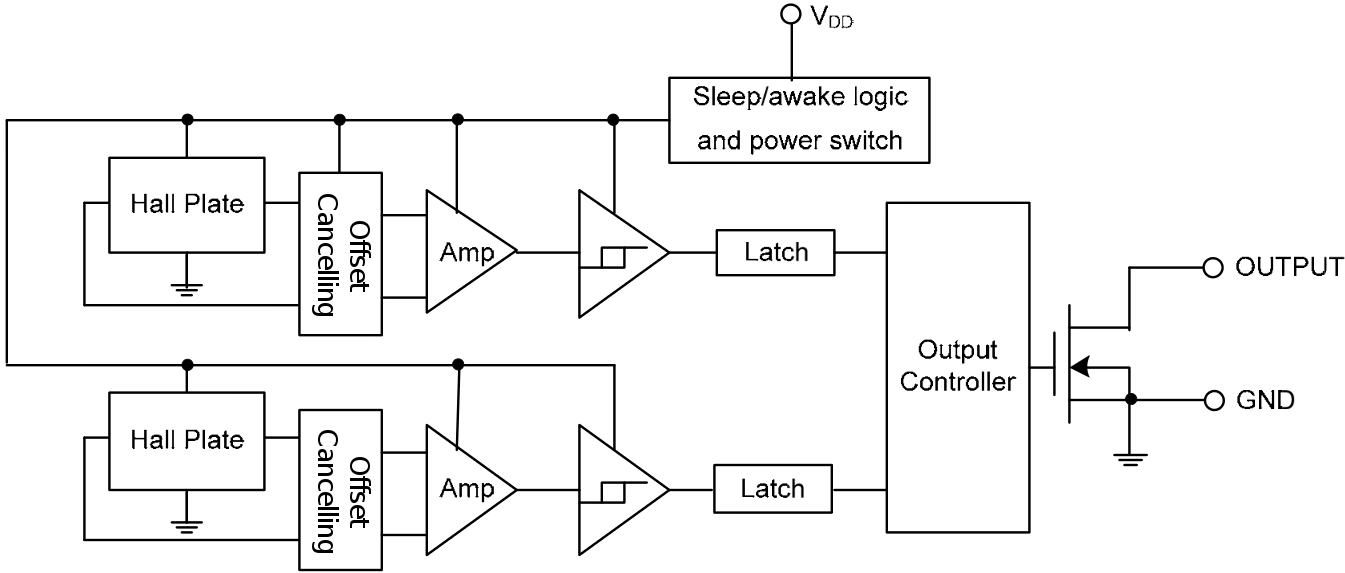
\includegraphics[width=0.75\textwidth]{\EtPath/Bilder/AH180N_functional.png}
	\caption{Funktionelles Blockschaltbild des Hall-Effekt-Schalters AH180N}
	\label{fig:AH180N_functional}
\end{figure}
\fi
%
\ifEMBED
\begin{figure}[h!]
	\centering
	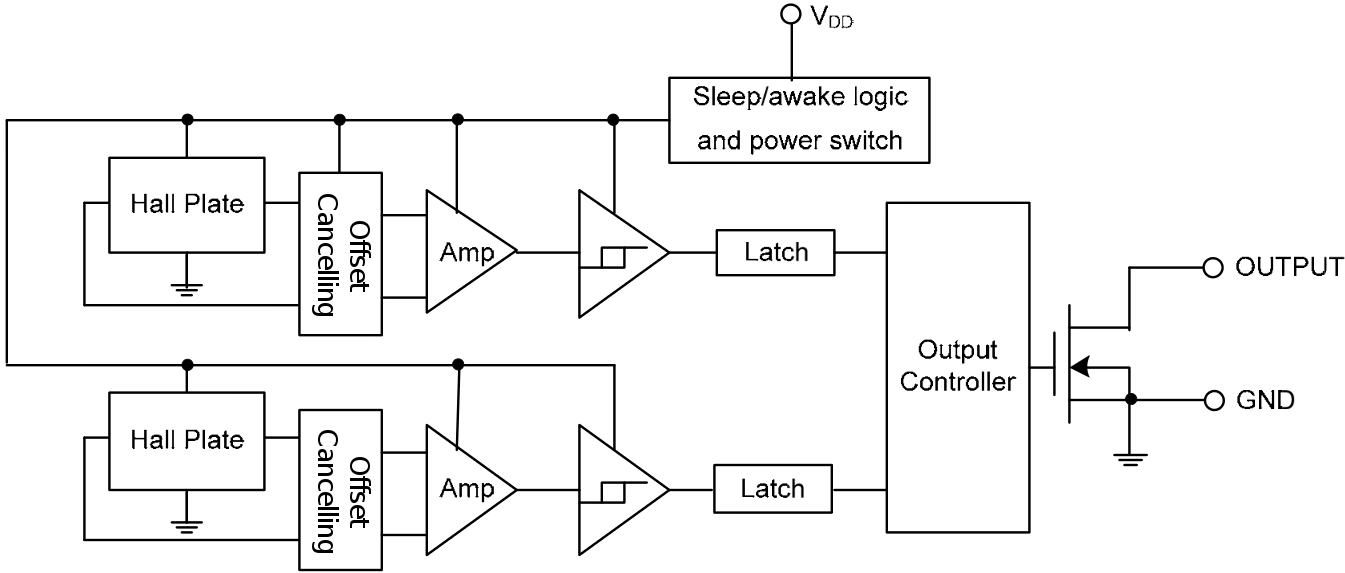
\includegraphics[width=0.75\textwidth]{\EtPath/Bilder/AH180N_functional.png}
	\caption{Funktionelles Blockschaltbild des Hall-Effekt-Schalters AH180N}
	\label{fig:AH180N_functional}
\end{figure}
\fi
%
Ein solches Verfahren lohnt sich bei schnellen Winkelgeschwindigkeiten
und ist für diesen Anwendungsfall sehr effizient. Zugehörige
Hall-Effekt-Schalter lassen sich einfach montieren und sind gegen Störungen
sehr robust. Ein mögliches Modell für einen Hall-Effekt-Schalter ist der
AH180N. Dieser bietet einen Open-Drain Ausgang, welcher somit logische Pegel
liefert (siehe Abbildung \ref{fig:AH180N_functional}). Interessant ist diese
Art von Drehzahl-Geber insbesondere durch ihren geringen Preis, denn solche
Hall-Effekt-Schalter, wie der AH180N, befinden sich im Preissegment von 
unter einem Franken.
\clearpage

\begin{flushleft}
    \renewcommand{\refname}{Literatur- und Quellenverzeichnis}
%        \{\refname}{Quellenverzeichnis}
    \bibliography{src/BLDC_Source}{} %!!! Kein Leerzeichen nach dem , !!!!
\end{flushleft}

\end{document}
